\documentclass{article}
\usepackage{graphicx}

\begin{document}

\title{Supplementary material for ``Visualization methods for RNA-sequencing data analysis"}
\author{Lindsay Rutter}

\maketitle

\begin{figure}[!p]
\centerline{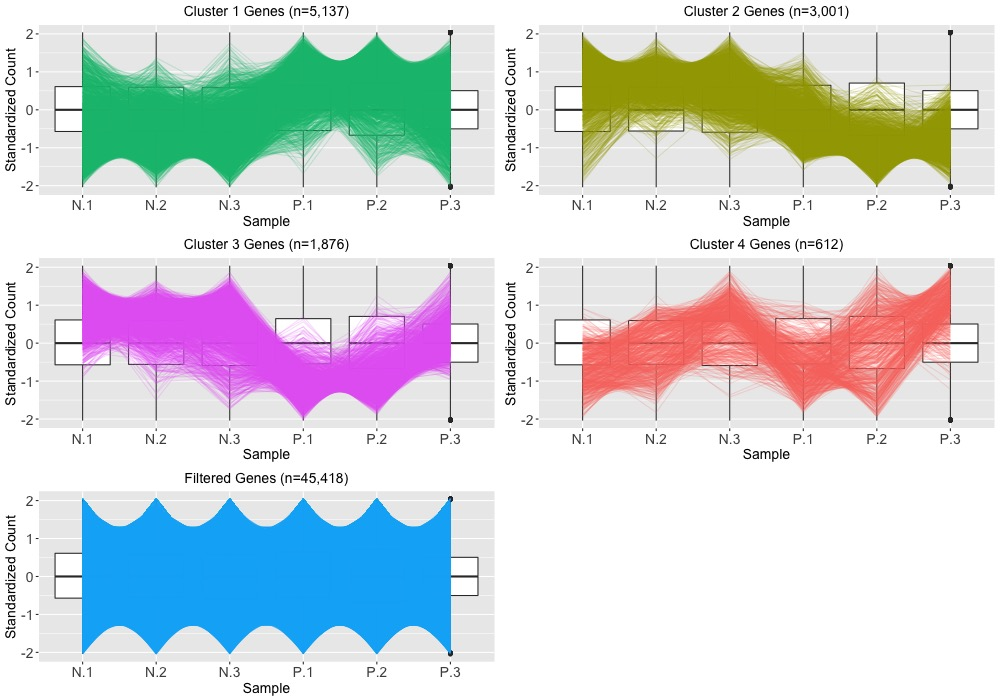
\includegraphics[width=\columnwidth]{/Users/lindz/JDSPaper/Bioinformatics/Pictures/FilterNotSig/ClusteringdataFDR05/NP4.jpg}}
\caption{Example application of parallel coordinate plots using the iron-metabolism soybean dataset. We filtered genes with low means and/or variance, performed a hierarchical clustering analysis with a cluster size of four, and visualized the results using parallel coordinate lines. Most non-filtered genes were in Clusters 1 and 2, which both showed overexpression in one treatment and underexpression in the other treatment. The genes in Cluster 4 mostly showed messy patterns with low signal to noise ratios. Interestingly, Cluster looked similar to Cluster 2 (large values for group N and small values for group P), except for unexpectedly large values for the third replicate of group P.
\label{suppNonSigCluster}}
\end{figure}

\begin{figure}[!p]
\centerline{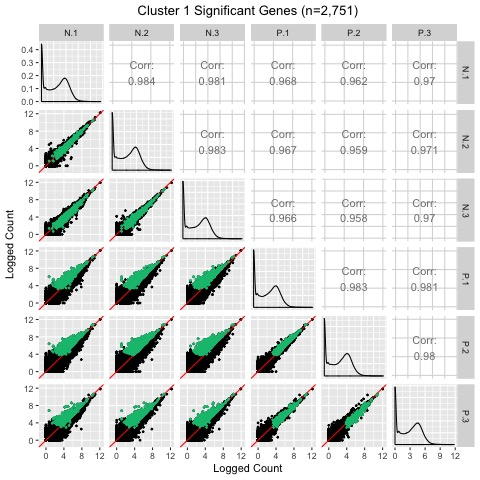
\includegraphics[width=\columnwidth]{/Users/lindz/JDSPaper/Bioinformatics/Pictures/FilterNotSig/Clustering_data_FDR_05/N_P_Sig_SM_4_1.jpg}}
\caption{Example of using a scatterplot matrix to assess DEG calls from a model in the iron-metabolism soybean dataset. There were 2751 significant genes in Cluster 1 after performing a hierarchical clustering analysis with a cluster size of four. These significant genes are overlaid in green over the scatterplot matrix. They follow the expected patterns of differential expression with most green points falling along the \textit{x=y} line in the scatterplots between replicates, but deviating from the \textit{x=y} line in the scatterplots between treatments. The deviation consistently demonstrates higher expression in the P group than in the N group. Hence, these green points seem to represent genes that were significantly overexpressed in the P group, which draws the same conclusion with what we derived using the parallel coordinate plots in Figure 2 of the paper. One difficulty with plotting such a large number of DEGs onto the scatterplot matrix is that overplotting can obscure our inability to determine how many DEGs are in a given location.
\label{suppSMCluster1}}
\end{figure}

\begin{figure}[!p]
\centerline{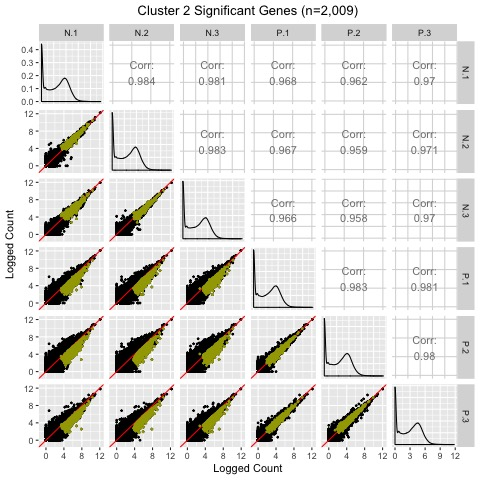
\includegraphics[width=\columnwidth]{/Users/lindz/JDSPaper/Bioinformatics/Pictures/FilterNotSig/Clustering_data_FDR_05/N_P_Sig_SM_4_2.jpg}}
\caption{Example of using a scatterplot matrix to assess DEG calls from a model in the iron-metabolism soybean dataset. There were 2009 significant genes in Cluster 2 after performing a hierarchical clustering analysis with a cluster size of four. These significant genes are overlaid in mustard over the scatterplot matrix. They follow the expected patterns of differential expression with most mustard points falling along the \textit{x=y} line in the scatterplots between replicates, but deviating from the \textit{x=y} line in the scatterplots between treatments. The deviation consistently demonstrates higher expression in the N group than in the P group. Hence, these mustard points seem to represent genes that were significantly overexpressed in the N group, which draws the same conclusion with what we derived using the parallel coordinate plots in Figure 2 of the paper. One difficulty with plotting such a large number of DEGs onto the scatterplot matrix is that overplotting can obscure our inability to determine how many DEGs are in a given location.
\label{suppSMCluster2}}
\end{figure}
  
\begin{figure}[!p]
\centerline{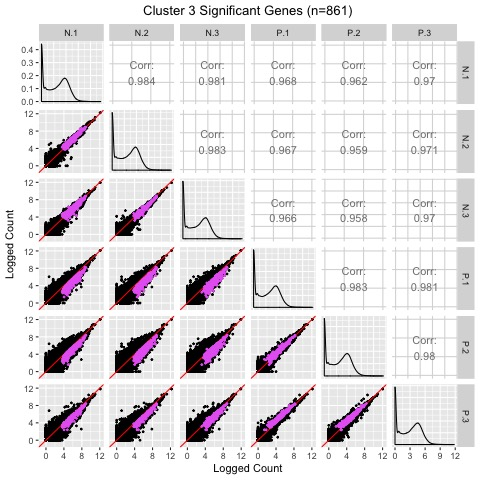
\includegraphics[width=\columnwidth]{/Users/lindz/JDSPaper/Bioinformatics/Pictures/FilterNotSig/Clustering_data_FDR_05/N_P_Sig_SM_4_3.jpg}}
\caption{Example of using a scatterplot matrix to assess DEG calls from a model in the iron-metabolism soybean dataset. There were 861 significant genes in Cluster 3 after performing a hierarchical clustering analysis with a cluster size of four. These significant genes are overlaid in pink over the scatterplot matrix. For the most part, they follow the expected patterns of differential expression with pink points falling along the \textit{x=y} line in the scatterplots between replicates, but deviating from the \textit{x=y} line in the scatterplots between treatments. The deviation consistently demonstrates higher expression in the N group than in the P group. However, the scatterplot between replicates P.1 and P.3 show slightly higher expression in P.3, and the scatterplot between replicates P.2 and P.3 also show slightly higher expression in P.3. Hence, these pink points seem to represent genes that were significantly overexpressed in the N group, but with slight inconstencies in the replicates in the P group. The parallel coordinate plots in Figure 2 of the paper showed this same conclusion and perhaps more clearly. One difficulty with plotting such a large number of DEGs onto the scatterplot matrix is that overplotting can obscure our inability to determine how many DEGs are in a given location.
\label{suppSMCluster3}}
\end{figure}  
  
\begin{figure}[!p]
\centerline{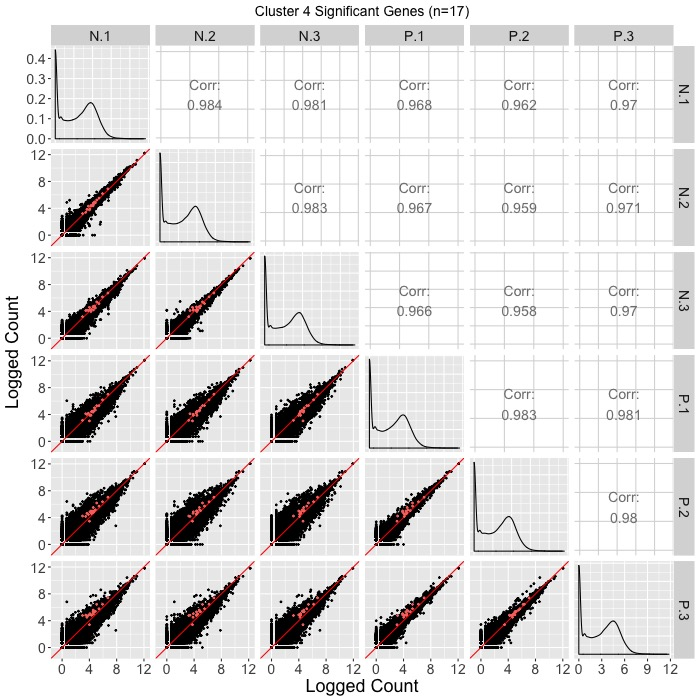
\includegraphics[width=\columnwidth]{/Users/lindz/JDSPaper/Bioinformatics/Pictures/FilterNotSig/Clustering_data_FDR_05/N_P_Sig_SM_4_4.jpg}}
\caption{Example of using a scatterplot matrix to assess DEG calls from a model in the iron-metabolism soybean dataset. There were 17 significant genes in Cluster 4 after performing a hierarchical clustering analysis with a cluster size of four. These significant genes are overlaid in coral over the scatterplot matrix. For the most part, they do not seem to follow the expected patterns of differential expression: In many of the scatterplots between treatments, the coral points do not seem to deviate much from the \textit{x=y} line. Moreover, in the scatterplots between P.1 and P.2 as well as P.1 and P.3, the coral points seems to indicate an underexpression of the P.1 replicate. We found a similar finding of somewhat messy looking DEG calls in Cluster 4 from Figure 2 in the paper. 
\label{suppSMCluster4}}
\end{figure}  
  
\begin{figure}[!p]
\centerline{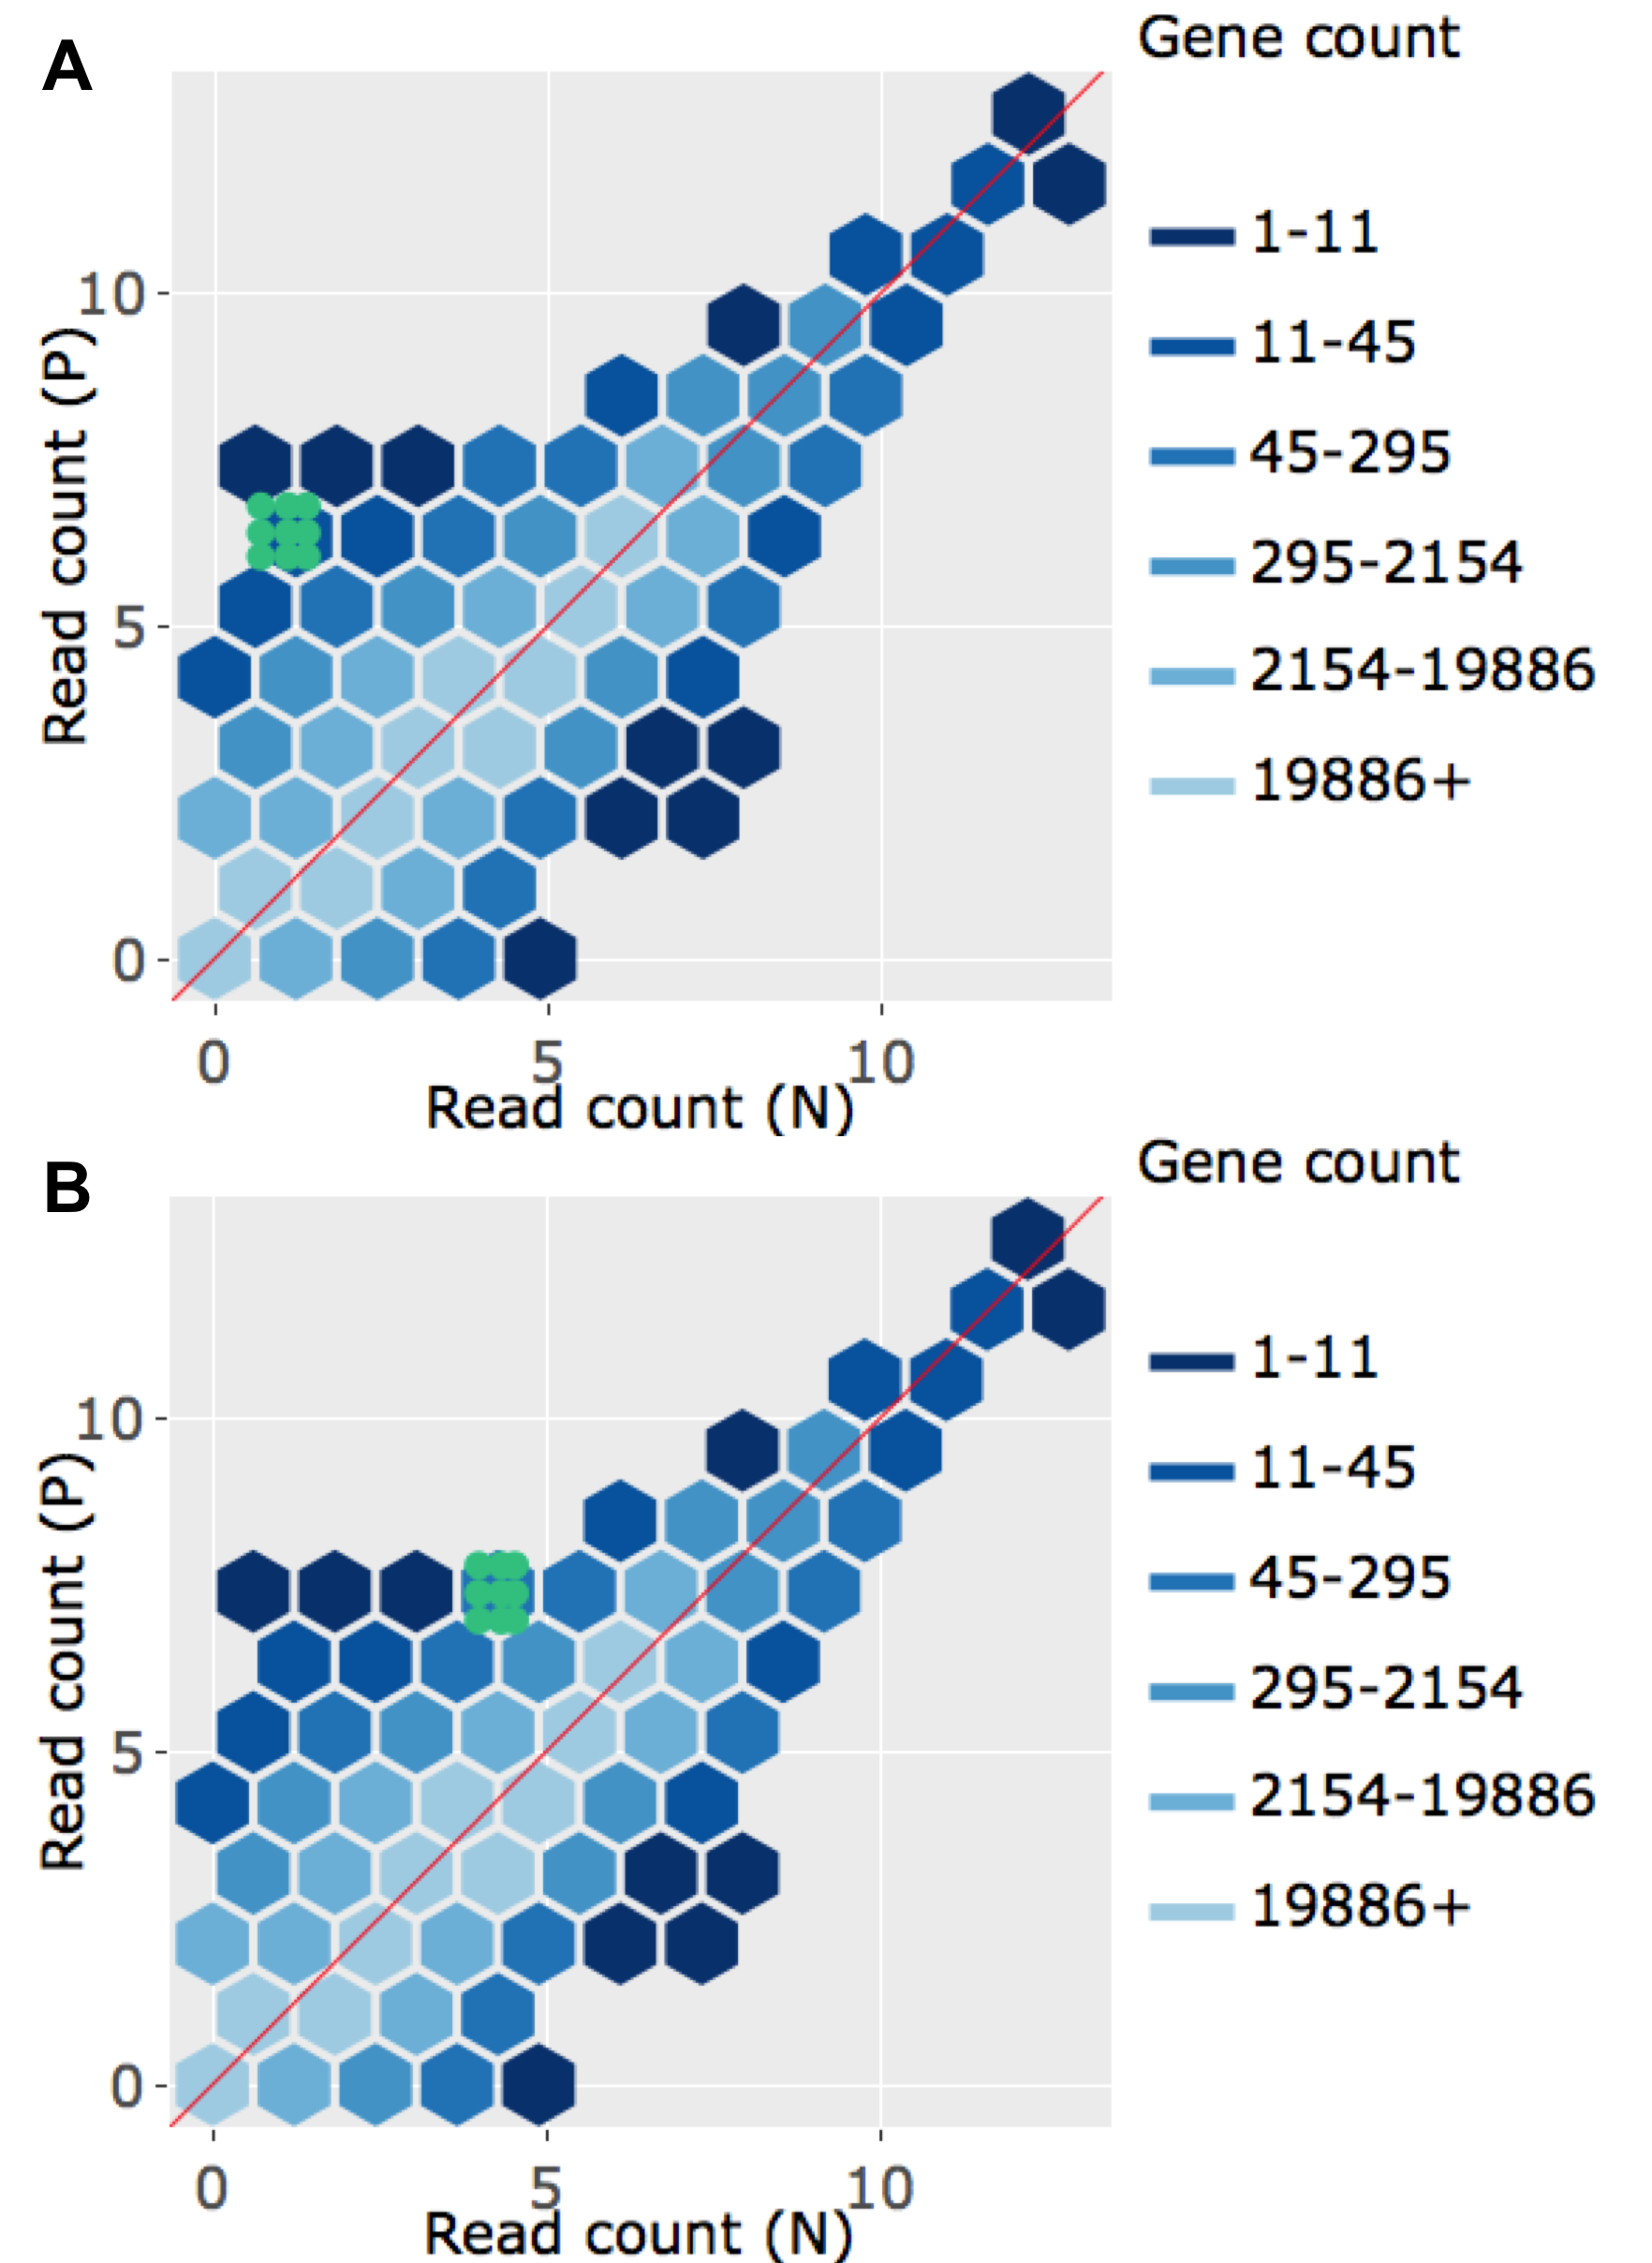
\includegraphics[width=0.7\columnwidth]{/Users/lindz/JDSPaper/Bioinformatics/Pictures/litrePlots/N_P/litreCluster1.png}}
\caption{Litre plots for significant genes inside Cluster 1 from Figure 2 of the paper. Subplots A and B each overlay a significant gene from Cluster 1 as nine green points. The genes show a pattern expected of a differentially-expressed one, by clumping together and deviating from the \textit{x=y} line. Moreover, the genes appear over-expressed in the P group. This is consistent with what we saw in Figure 2 of the paper. To interactively view the litre plot for all significant genes within Cluster 1, please visit https://rnaseqvisualization.shinyapps.io/litreCluster1.
\label{litreCluster1}}
\end{figure}   

\end{document}